\documentclass{article}
\usepackage{xcolor}
\usepackage{titleps}
\usepackage[letterpaper, margin=0.95in]{geometry}
\usepackage{url}
\usepackage{amsmath}
\usepackage{amssymb}
\usepackage{wrapfig}
\usepackage{float}
\usepackage{mathtools}
\usepackage{enumitem}
\usepackage{tabu}
\usepackage{parskip}
\usepackage{natbib}
\usepackage{listings}
\usepackage{tikz}
\usepackage{quiver}

\newcommand{\xb}{\mathbf{x}}
\newcommand{\yb}{\mathbf{y}}
\newcommand{\wb}{\mathbf{w}}
\newcommand{\Xb}{\mathbf{X}}
\newcommand{\Yb}{\mathbf{Y}}
\newcommand{\tr}{^T}
\newcommand{\hb}{\mathbf{h}}
\newcommand{\Hb}{\mathbf{H}}

\DeclareFontShape{OT1}{cmtt}{bx}{n}{<5><6><7><8><9><10><10.95><12><14.4><17.28><20.74><24.88>cmttb10}{}


\usepackage{forest}

\usepackage{hyperref}
\usepackage[color=red]{todonotes}
\usepackage{forest}
\definecolor{light-yellow}{HTML}{FFE5CC}

\usepackage{cleveref}

\newpagestyle{ruled}
{\sethead{Berkeley CS 285}{Deep Reinforcement Learning, Decision Making, and Control}{Fall 2023}\headrule
  \setfoot{}{}{}}
\pagestyle{ruled}

\renewcommand\makeheadrule{\color{black}\rule[-.75\baselineskip]{\linewidth}{0.4pt}}
\renewcommand*\footnoterule{}

\begin{document}
\lstset{basicstyle = \ttfamily,columns=fullflexible,
backgroundcolor = \color{light-yellow}
}

\begin{centering}
    {\Large [SOLUTION TEMPLATE] Assignment 2: Policy Gradients} \\
    \vspace{.25cm}
    \textbf{Due September 25, 11:59 pm} \\
\end{centering}

\setcounter{section}{3}
\section{Policy Gradients}
\begin{itemize}
\item Create two graphs:
\begin{itemize}
\item In the first graph, compare the learning curves (average return vs. number of environment steps) for the experiments prefixed with \verb|cartpole|. (The small batch experiments.)
\item In the second graph, compare the learning curves for the experiments prefixed with \verb|cartpole_lb|. (The large batch experiments.)
\end{itemize}
\begin{enumerate}[]
	\item The learning curves for \verb|cartpole_lb| small batch experments are as following: 
		\begin{figure}[ht]
			\centering
			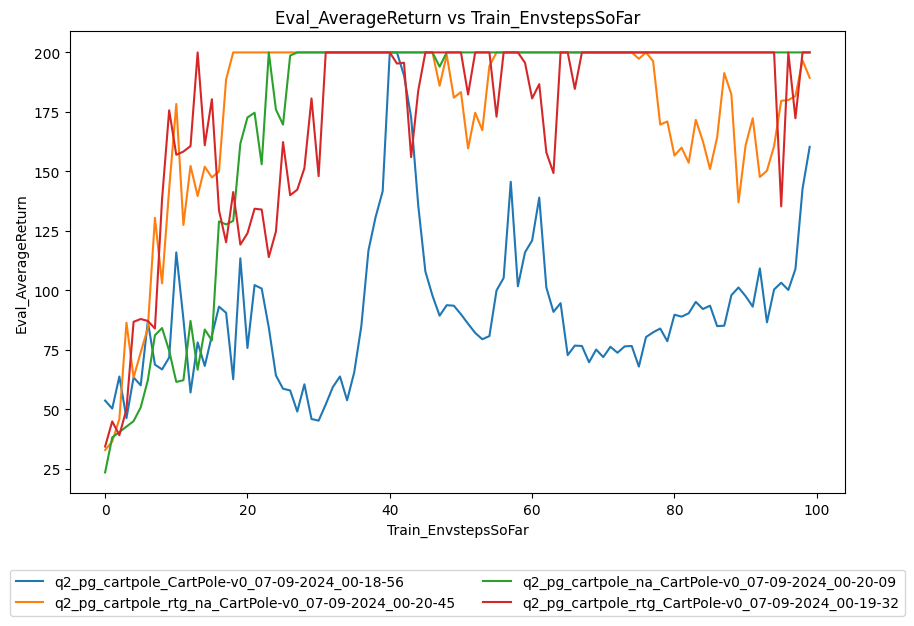
\includegraphics[width=0.6\textwidth]{./images/4-CartPole-small.png}
			\caption{Learning Curve : CartPole-small}
			\label{fig:CartPole-small}
		\end{figure}
	\item The learning curves for \verb|cartpole_lb| large batch experments are as following:
		\begin{figure}[ht]
			\centering
			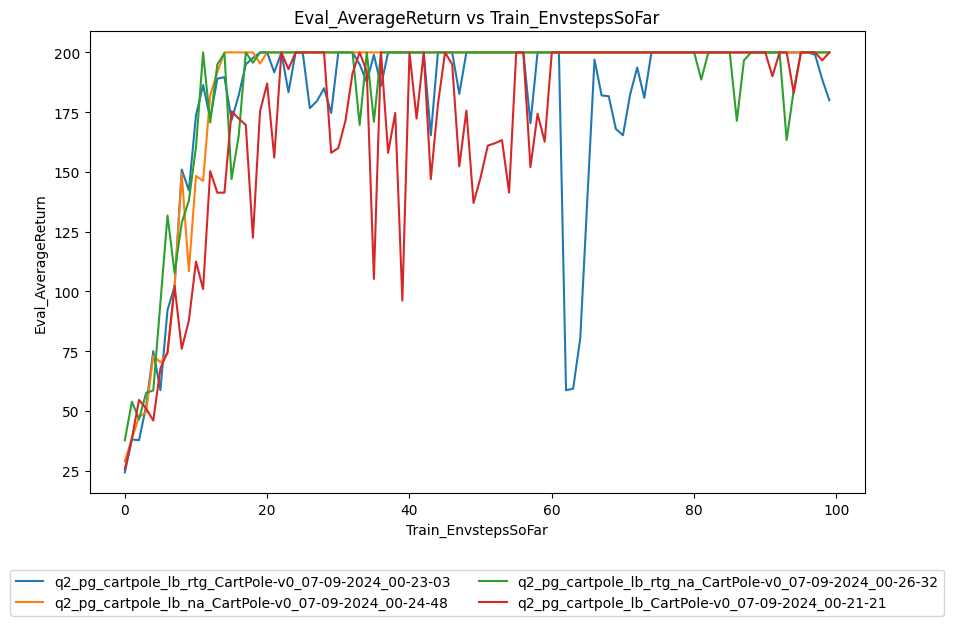
\includegraphics[width=0.6\textwidth]{./images/4-CartPole-large.png}
			\caption{Learning Curve : CartPole-large}
			\label{fig:CartPole-large}
		\end{figure}
\end{enumerate}
\textbf{For all plots in this assignment, the $x$-axis should be number of environment steps, logged as} \verb|Train_EnvstepsSoFar| \textbf{(\textit{not} number of policy gradient iterations).}
\item Answer the following questions briefly: 
\begin{itemize}
\item Which value estimator has better performance without advantage normalization: the trajectory-centric one, or the one using reward-to-go?

\textbf{Solution:} \textit{The Reward-to-Go value estimator performs better without normalization.}

\item Did advantage normalization help?

	\textbf{Solution:} \textit{Yes, normalization process helped.  For trajectory-centric one, normalized one learned faster and reduced variance. For reward-to-go, it improves learning speed. }

\item Did the batch size make an impact?

	\textbf{Solution:} \textit{Yes, larger batch size generally better, while normalized reward-to-go performed roughly same.}

\end{itemize}
\item Provide the exact command line configurations (or \texttt{\#@params} settings in Colab) you used to run your experiments, including any parameters changed from their defaults.
\end{itemize}

\newpage\section{Neural Network Baseline}
\begin{itemize}
    \item Plot a learning curve for the baseline loss.
		\begin{figure}[ht]
			\centering
			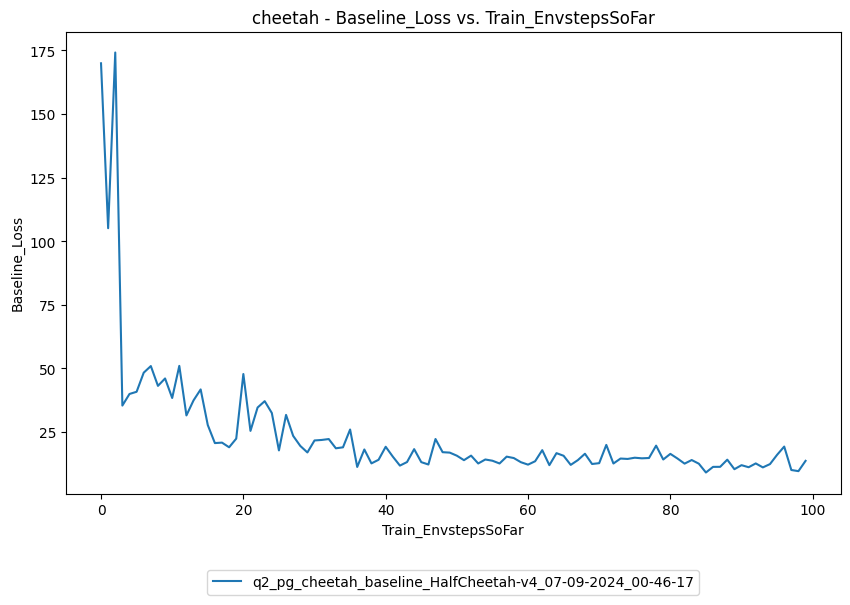
\includegraphics[width=0.6\textwidth]{./images/5-HalfCheetah-baseline_loss.png}
			\caption{Learning Curve : HalfCheetah-Baseline loss}
			\label{fig:HalfCheetah-baseline_loss}
		\end{figure}
    \item Plot a learning curve for the eval return. You should expect to achieve an average return over 300 for the baselined version.
		\begin{figure}[ht]
			\centering
			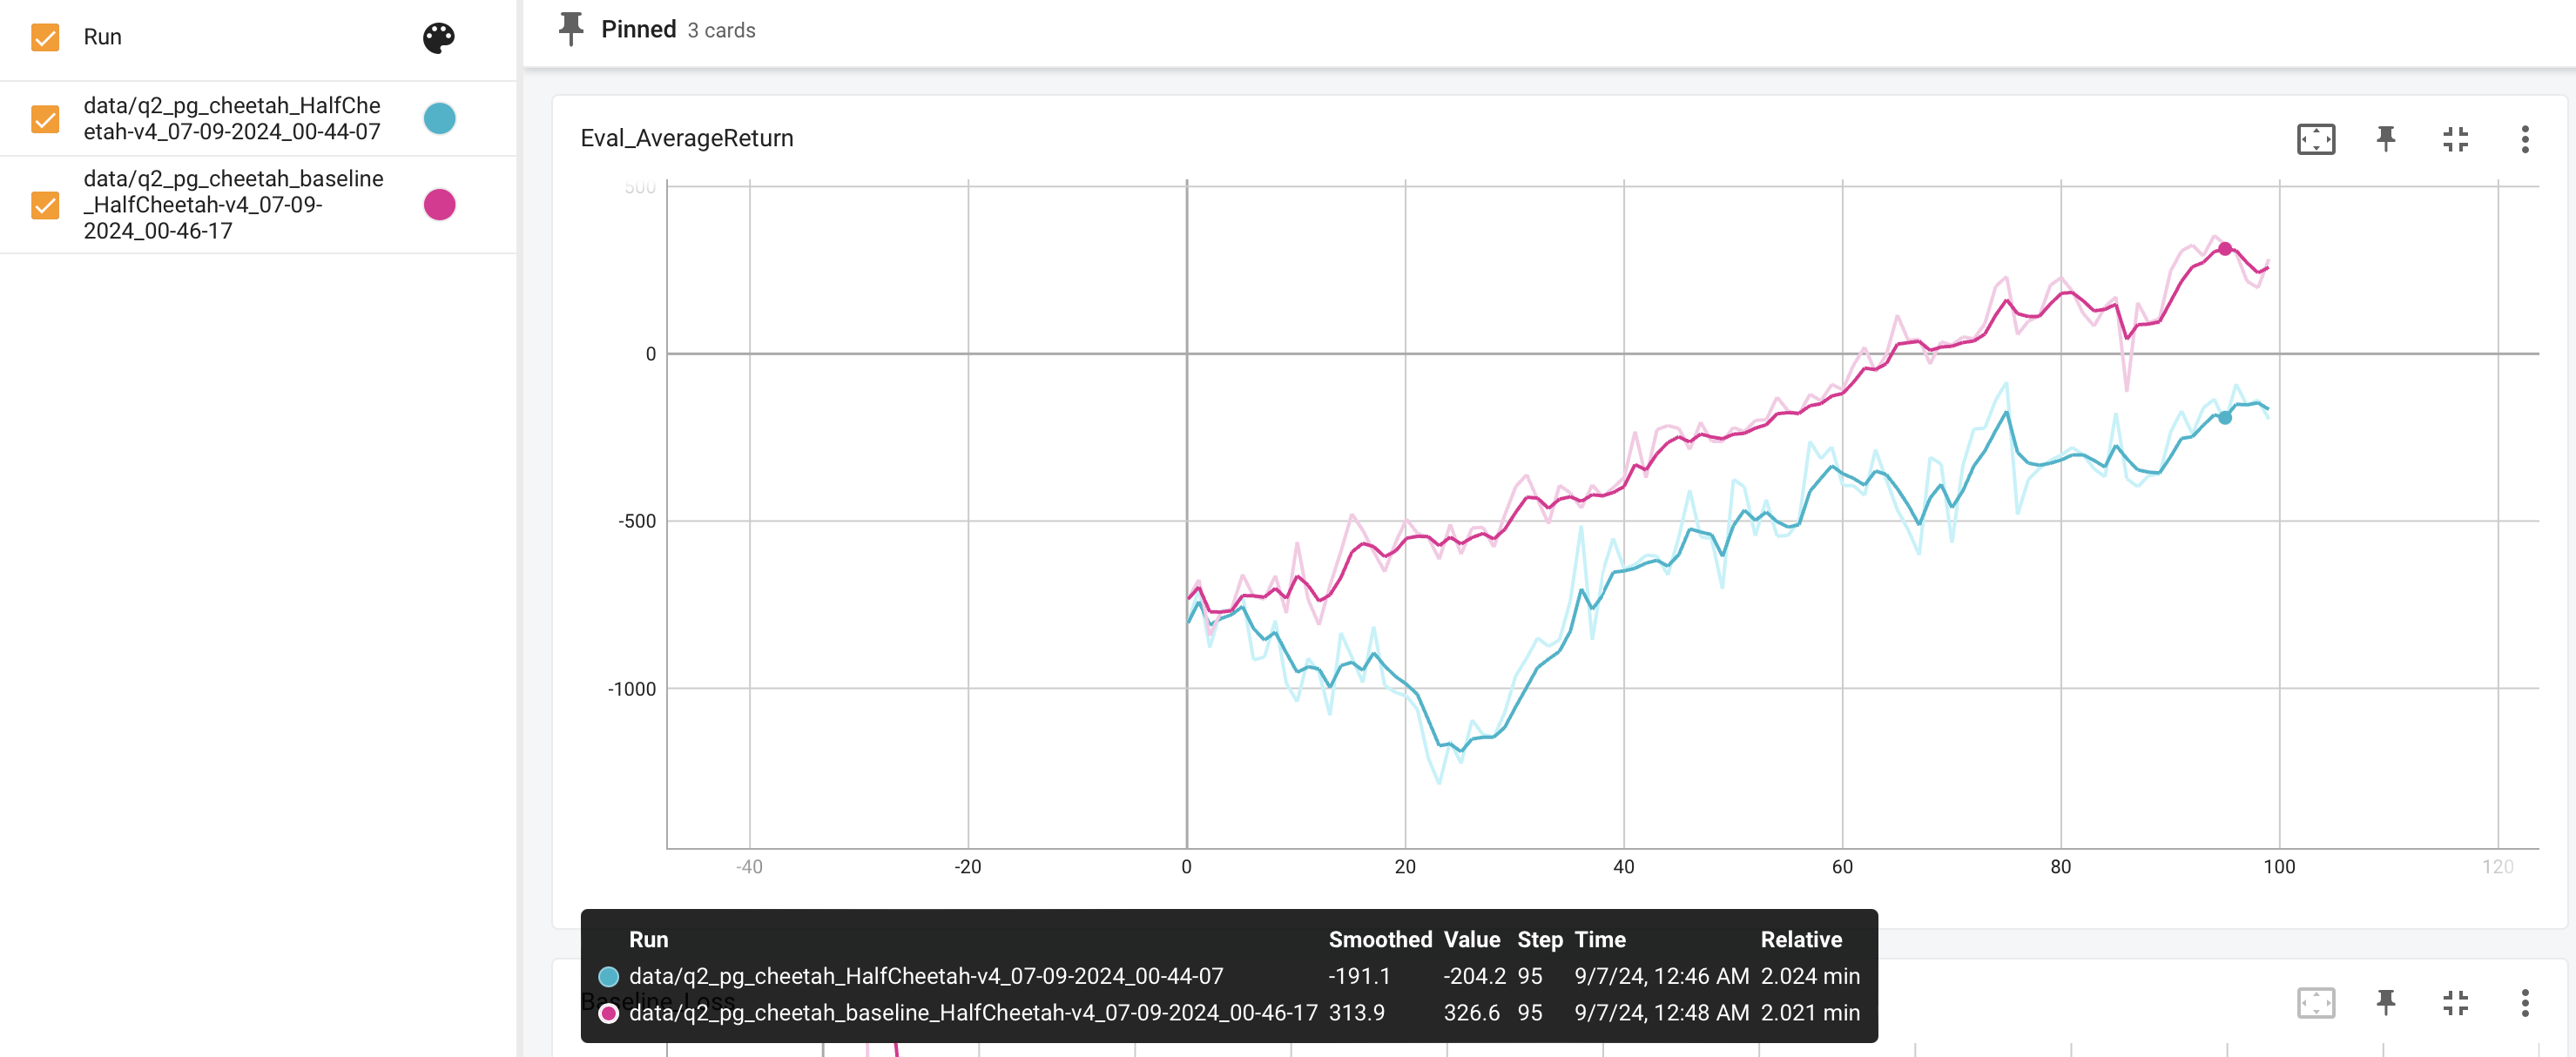
\includegraphics[width=0.8\textwidth]{./images/5-HalfCheetah-learning_curve.png}
			\caption{Learning Curve : HalfCheetah-Learning Curve}
			\label{fig:HalfCheetah-Learning_Curve}
		\end{figure}
    \item Run another experiment with a decreased number of baseline gradient steps (\verb|-bgs|) and/or baseline learning rate (\verb|-blr|). How does this affect (a) the baseline learning curve and (b) the performance of the policy?
    
    \textbf{Solution:} 
    \begin{itemize}
    	\item \textit{The baseline loss in both decreased number of baseline gradient steps and baseline learning rate is performs higher loss, but losses converge to roughly same level to non-decreased one after around $40$ steps.}
    	\item \textit{While decreased number of baseline gradient steps and baseline learning rate returned poorer performance in learning curve.}
    \end{itemize}
    
    \item \textbf{Optional:} Add \verb|-na| back to see how much it improves things. Also, set \verb|video_log_freq 10|, then open TensorBoard and go to the ``Images'' tab to see some videos of your HalfCheetah walking along!
    
    \textbf{Solution:} 
    \item \textit{The normalization helps with improving learning performance, while baseline loss keeps at the same level while becomes more stable (i.e. smoother).}
    
    
\end{itemize}

\newpage\section{Generalized Advantage Estimation}
\begin{itemize}
    \item Provide a single plot with the learning curves for the \verb|LunarLander-v2| experiments that you tried. Describe in words how $\lambda$ affected task performance. The run with the best performance should achieve an average score close to 200 (180+).
    \begin{figure}[ht]
    	\centering
    	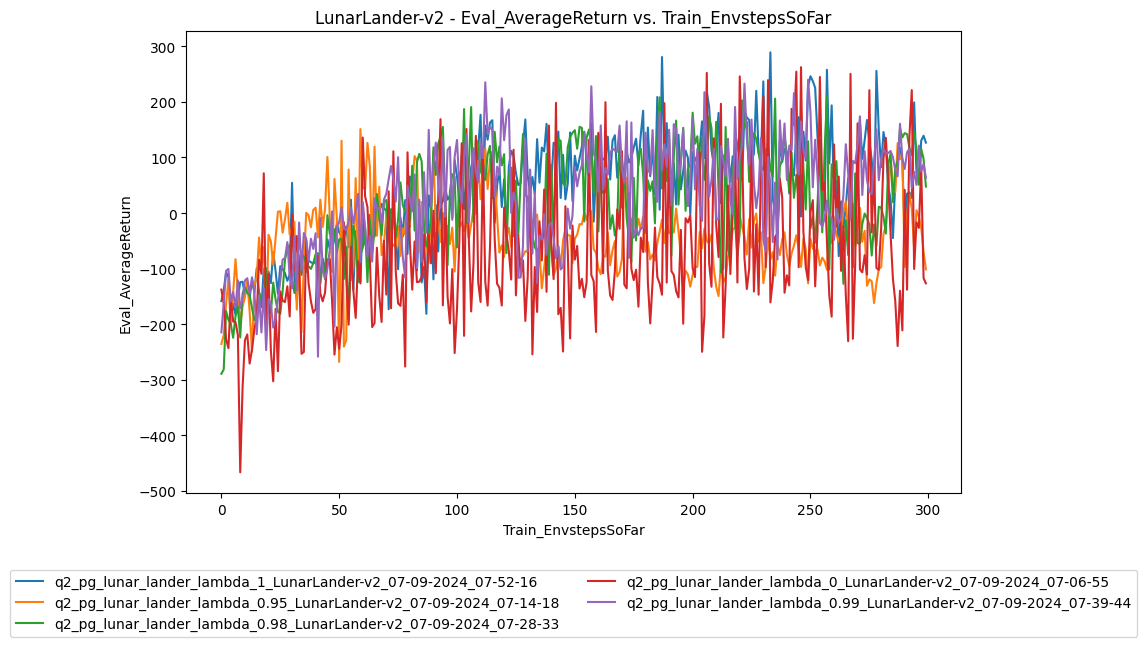
\includegraphics[width=0.9\textwidth]{./images/6-LunarLander-LearningCurve.png}
    	\caption{LunarLander: Learning Curve}
    	\label{fig:6-LunarLander-LearningCurve}
    \end{figure}
    \item Consider the parameter $\lambda$. What does $\lambda = 0$ correspond to? What about $\lambda = 1$? Relate this to the task performance in \verb|LunarLander-v2| in one or two sentences.
    
    \begin{itemize}
	   \item When $\lambda=0$, GAE becomes $A_{GAE}^{\pi}(s_t, a_t)=\delta_t (s_t, a_t)=r(s_t, a_t) + \gamma V_{\phi}^{\pi}(s_{t+1}) - V_{\phi}^{\pi}(s_t)$, which is equivalent of single-step advantage estimator, with low-variance and high-bias.
    
	    \item When $\lambda=1$, GAE becomes  $A_{GAE}^{\pi}(s_t, a_t)=\sum_{t'=t}^{T-1}\gamma^{t'-t}\delta_{t'}$, which is the multi-step actor critic method, with high variance and low bias.
	\end{itemize}
\end{itemize}

\newpage\section{Hyperparameter Tuning}
\begin{enumerate}
    \item Provide a set of hyperparameters that achieve high return on \verb|InvertedPendulum-v4| in as few environment steps as possible.
    \item Show learning curves for the average returns with your hyperparameters and with the default settings, with environment steps on the $x$-axis. Returns should be averaged over 5 seeds.
     \begin{figure}[ht]
    	\centering
    	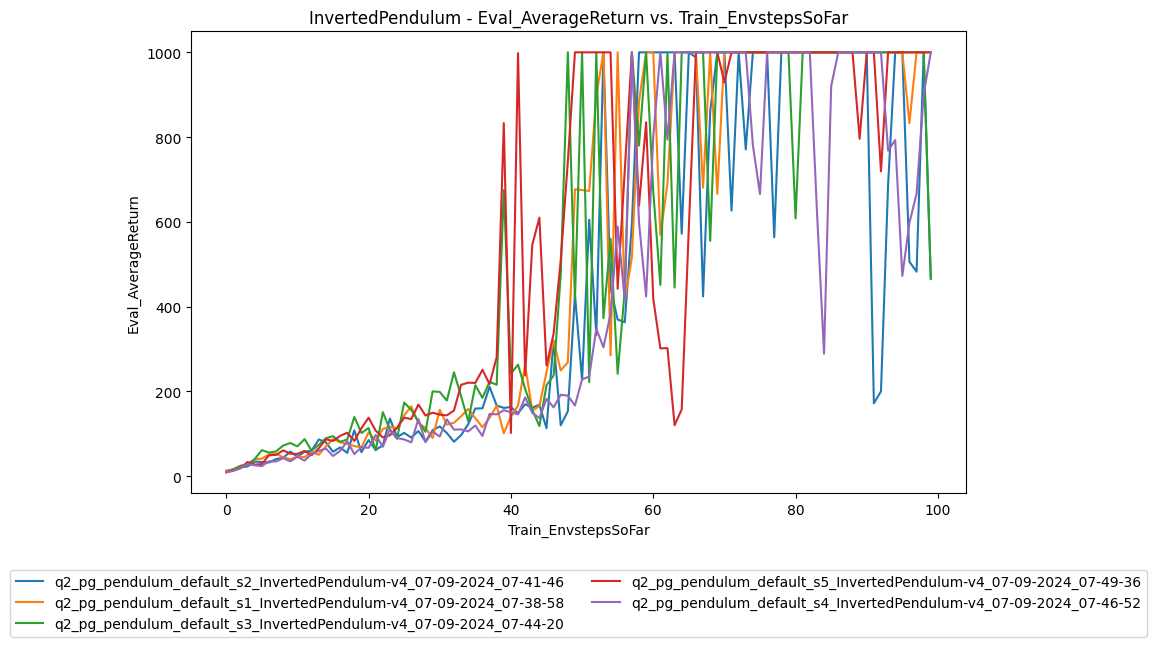
\includegraphics[width=0.9\textwidth]{./images/7-InvertedPendulum-LearningCurve.png}
    	\caption{InvertedPendulum: Learning Curve}
    	\label{fig:7-InvertedPendulum-LearningCurve}
    \end{figure}
\end{enumerate}

\newpage\section{(Extra Credit) Humanoid}
\begin{enumerate}
    \item Plot a learning curve for the Humanoid-v4 environment. You should expect to achieve an average return of at least 600 by the end of training. Discuss what changes, if any, you made to complete this problem (for example: optimizations to the original code, hyperparameter changes, algorithmic changes).
     \begin{figure}[ht]
    	\centering
    	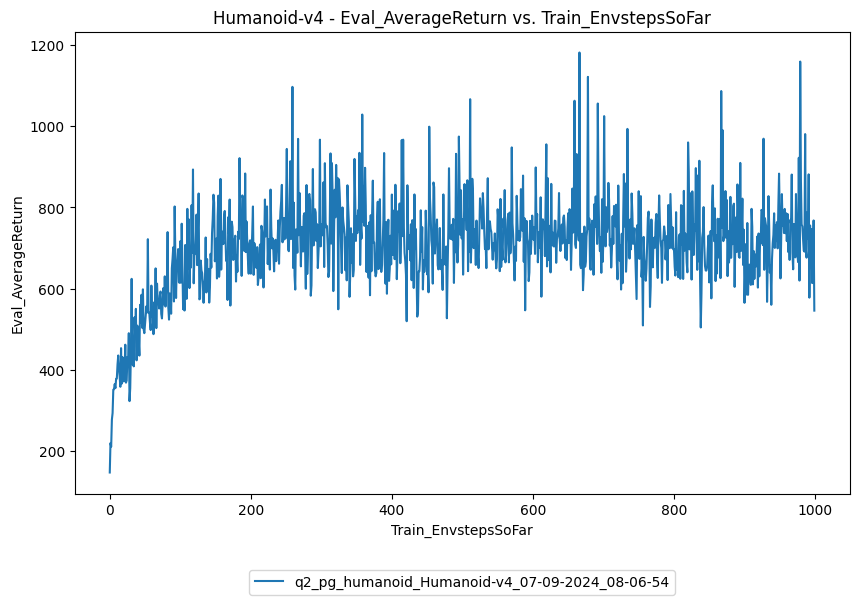
\includegraphics[width=0.9\textwidth]{./images/8-Humanoid-LearningCurve.png}
    	\caption{Humanoid: Learning Curve}
    	\label{fig:8-Humanoid-LearningCurve}
    \end{figure}
\end{enumerate}

\newpage\section{Analysis}
\label{sec:analysis}
Consider the following infinite-horizon MDP:
% https://q.uiver.app/#q=WzAsMixbMCwwLCJzIl0sWzAsMSwic19GIl0sWzAsMSwiYV8yIl1d
\[\begin{tikzcd}
	s_1 & {s_F}
	\arrow["{a_2}", from=1-1, to=1-2]
    \arrow["{a_1}", loop left, from=1-1, to=1-1]
\end{tikzcd}\]
\newcommand{\Rmax}[0]{R_{\textrm{max}}}
\newcommand{\E}[0]{\mathbb{E}}
\newcommand{\var}[0]{\textrm{Var}}
\crefname{question}{part}{parts}
\Crefname{question}{Part}{Parts}
\newcommand\question[1][]{\item\refstepcounter{subsection}\label[question]{#1}}

At each step, the agent stays in state $s_1$ and receives reward 1 if it takes action $a_1$, and receives reward 0 and terminates the episode otherwise.
Parametrize the policy as stationary (not dependent on time) with a single parameter:
\[\pi_\theta(a_1|s_1) = \theta, \pi_\theta(a_2|s_1) = 1-\theta\]

\begin{enumerate}
\question[sec:analysis1] Applying policy gradients
\begin{enumerate}
    \item Use policy gradients to compute the gradient of the expected return $R(\tau)$ with respect to the parameter $\theta$. \textbf{Do not use discounting.}

    \textbf{Hint}: to compute $\sum_{k=1}^\infty k\alpha^{k-1}$, you can write:
    \[\sum_{k=1}^\infty k\alpha^{k-1} = \sum_{k=1}^\infty \frac{d}{d\alpha}\alpha^k = \frac{d}{d\alpha}\sum_{k=1}^\infty\alpha^k\]

\textbf{Solution:}
	In this setting, each episode can continue indefinitely (since we are not using discounting), but at each step, there’s a chance the agent terminates the episode.
	Due to $\pi_{\theta}$ is parameterized by $\theta$, and $\pi_{\theta}(a_1 | s_1) = \theta$, $\pi_{\theta}(a_2 | s_1) = 1- \theta$, then:
		$$\begin{aligned}
			J(\theta) &= \sum_{k=1}^{\infin} \rm Pr(\text{survive for k steps}) \times 1 \\
			&= \sum_{k=1}^{\infin} \theta^k \\
			&= \frac{\theta}{1 - \theta} \\
		\end{aligned}$$
	Take the gradient with respect to $\theta$: 
		$$
			\nabla_\theta  J(\theta) = \frac{1}{(1 - \theta) ^ 2}
		$$
		
    \item \label{exact_gradient} Compute the expected return of the policy $\E_{\tau \sim \pi_\theta} R(\tau)$ directly. Compute the gradient of this expression with respect to $\theta$ and verify that this matches the policy gradient.

\textbf{Solution:}

		\[	\mathbb{E}_{\tau \sim \pi_\theta} R(\tau) &= J(\theta) \]
		\[\nabla_\theta \mathbb{E}_{\tau \sim \pi_\theta} R(\tau) &=  \frac{1}{(1 - \theta) ^ 2}\]
			

\end{enumerate}
\newpage
\question[sec:analysis2] Compute the variance of the policy gradient in closed form and describe the properties of the variance with respect to $\theta$. For what value(s) of $\theta$ is variance minimal? Maximal? (Once you have an exact expression for the variance you can eyeball the min/max).

\textbf{Hint:}  Once you have it expressed as a sum of terms $P(\theta)/Q(\theta)$ where $P$ and $Q$ are polynomials, you can use a symbolic computing program (Mathematica, SymPy, etc) to simplify to a single rational expression.

\textbf{Solution:}

To compute the variance of the policy gradient in closed form, we first need to express the policy gradient and its associated variance mathematically.

### Step 1: Recall the policy gradient

The expected return is given by:

\[
J(\theta) = \frac{\theta}{1 - \theta}
\]

The policy gradient is:

\[
\nabla_\theta J(\theta) = \frac{1}{(1 - \theta)^2}
\]

### Step 2: Variance of the policy gradient

The variance of the policy gradient refers to the variability in the gradient estimates over different episodes. For simplicity, let’s compute the variance of a simple case where each episode either continues with probability \( \theta \) or terminates with probability \( 1 - \theta \).

The reward \( R \) in each episode is the number of steps the agent survives (each survival step gives a reward of 1). The probability of surviving for \( k \) steps and then terminating is:

\[
\Pr(\text{survive } k \text{ steps}) = (1 - \theta)\theta^{k-1}
\]

Thus, the expected return is the sum over all possible episode lengths:

\[
J(\theta) = \sum_{k=1}^{\infty} k (1 - \theta) \theta^{k-1} = \frac{\theta}{(1 - \theta)^2}
\]

To compute the variance, we need the second moment of the return, \( \mathbb{E}[R^2] \), where \( R \) is the episode length.

The probability of surviving for \( k \) steps is \( (1 - \theta) \theta^{k-1} \), so the second moment is:

\[
\mathbb{E}[R^2] = \sum_{k=1}^{\infty} k^2 (1 - \theta) \theta^{k-1}
\]

This can be computed using a known formula for sums of this type:

\[
\sum_{k=1}^{\infty} k^2 \alpha^k = \frac{\alpha(1 + \alpha)}{(1 - \alpha)^3}, \quad \text{for } |\alpha| < 1
\]

Using \( \alpha = \theta \), the second moment is:

\[
\mathbb{E}[R^2] = \frac{\theta(1 + \theta)}{(1 - \theta)^3}
\]

### Step 3: Compute the variance

The variance of \( R \), \( \text{Var}(R) \), is given by:

\[
\text{Var}(R) = \mathbb{E}[R^2] - (\mathbb{E}[R])^2
\]

Substituting the expressions for \( \mathbb{E}[R^2] \) and \( \mathbb{E}[R] \):

\[
\text{Var}(R) = \frac{\theta(1 + \theta)}{(1 - \theta)^3} - \left( \frac{\theta}{(1 - \theta)^2} \right)^2
\]

Simplifying the right-hand side:

\[
\text{Var}(R) = \frac{\theta(1 + \theta)}{(1 - \theta)^3} - \frac{\theta^2}{(1 - \theta)^4}
\]

### Step 4: Find the minimum and maximum of the variance

To find the values of \( \theta \) where the variance is minimized and maximized, we analyze the expression:

\[
\text{Var}(R) = \frac{\theta(1 + \theta)}{(1 - \theta)^3} - \frac{\theta^2}{(1 - \theta)^4}
\]

1. **At \( \theta = 0 \):**
\[
\text{Var}(R) = 0
\]
This makes sense because if \( \theta = 0 \), the agent always terminates after 1 step, so there is no variance in the returns.

2. **At \( \theta = 1 \):**
\[
\text{Var}(R) = \infty
\]
This also makes sense because if \( \theta = 1 \), the agent never terminates, and the episode length could become infinitely large, resulting in infinite variance.

3. **For intermediate values of \( \theta \):**
The variance increases as \( \theta \) increases from 0 to 1, and the variance becomes maximal near \( \theta = 1 \).

### Conclusion:

- The **minimal variance** occurs at \( \theta = 0 \), where the policy deterministically terminates the episode after 1 step.
- The **maximal variance** occurs as \( \theta \) approaches 1, where the agent almost never terminates, leading to highly variable episode lengths.



\newpage
\question[sec:analysis3] Apply return-to-go as an advantage estimator.
\begin{enumerate}
    \item Write the modified policy gradient and confirm that it is unbiased.

\textbf{Solution:}

    \item Compute the variance of the return-to-go policy gradient and plot it on $[0, 1]$ alongside the variance of the original estimator.

\textbf{Solution:}

\end{enumerate}
\newpage
\question[sec:analysis4] Consider a finite-horizon $H$-step MDP with sparse reward:
% https://q.uiver.app/#q=WzAsNixbMCwwLCJzXzEiXSxbMSwwLCJzXzIiXSxbMiwwLCJzXzMiXSxbMiwxLCJzX0YiXSxbMywwLCJcXGRvdHMiXSxbNCwwLCJzX0giXSxbMCwxLCJhXzEiXSxbMSwyLCJhXzEiXSxbMCwzLCJhXzIiLDJdLFsyLDQsImFfMSJdLFs0LDVdLFsxLDMsImFfMiJdLFsyLDMsImFfMiIsMV0sWzQsMywiYV8yIiwxXV0=
\[\begin{tikzcd}
	{s_1} & {s_2} & {s_3} & \dots & {s_H} \\
	&& {s_F}
	\arrow["{a_1}", from=1-1, to=1-2]
	\arrow["{a_1}", from=1-2, to=1-3]
	\arrow["{a_2}"', from=1-1, to=2-3]
	\arrow["{a_1}", from=1-3, to=1-4]
	\arrow[from=1-4, to=1-5]
	\arrow["{a_2}", from=1-2, to=2-3]
	\arrow["{a_2}"{description}, from=1-3, to=2-3]
	\arrow["{a_2}"{description}, from=1-4, to=2-3]
\end{tikzcd}\]

The agent receives reward $\Rmax$ if it arrives at $s_H$ and reward $0$ if it arrives at $s_F$ (a terminal state). In other words, the return for a trajectory $\tau$ is given by:
\[R(\tau) = \begin{cases}1 & \tau \textrm{ ends at } s_H \\ 0 & \tau \textrm{ ends at } s_F \end{cases}\]
Using the same policy parametrization as above, consider off-policy policy gradients via importance sampling. Assume we want to compute policy gradients for a policy $\pi_\theta$ with samples drawn from $\pi_{\theta'}$.
\begin{enumerate}
    \item Write the policy gradient with importance sampling.

    \item Compute its variance.

\end{enumerate}

\end{enumerate}

\newpage\section{Survey}
\label{sec:survey}
Please estimate, in minutes, for each problem, how much time you spent (a) writing code and (b) waiting for the results. This will help us calibrate the difficulty for future homeworks. 
\begin{itemize}
    \item \textbf{Policy Gradients:}
    \item \textbf{Neural Network Baseline:}
    \item \textbf{Generalized Advantage Estimation:}
    \item \textbf{Hyperparameters and Sample Efficiency:}
    \item \textbf{Humanoid:}
    \item \textbf{Humanoid:}
    \item \textbf{Analysis -- applying policy gradients:}
    \item \textbf{Analysis -- PG variance:}
    \item \textbf{Analysis -- return-to-go:}
    \item \textbf{Analysis -- importance sampling:}
\end{itemize}

\end{document}
